\documentclass{article}

\begin{document}
\section{Simulation}
Computer simulation of continuous mathematical equations need to account for the fact that computers can only represent quanitities with finite accuracy. This is achieved by discretizing time and space into a grid, and applying adequate methods to step between the points in the grid by using current values to estimate values at the next position.

\subsection{Finite Difference}

The finite difference methods for stepping through space are based on the Taylor series expansion of the function:

$$f(x+h) = \sum_{n=0}^\infty \frac{h^n}{n!}f^{(n)}(x)$$

Truncating the series after the n-th element adds an error of order $O(h^{(n)})$ [O-notation] to the approximation and applying the truncation for example after n=2 results in 

$$f(x+h)=f(x)+hf'(x)+O(h^2)$$

Which suggests a discrete-time approximation for the derivative of $f(x)$:

$$f'(x)=\frac{f(x+h)-f(x)}{h}+O(h)$$

Which is known as the forward-difference. Other variants are central- (a) and backward-difference (b):

$$f'(x)=\frac{f(x+h)-f(x-h)}{2h}+O(h^2)$$

$$f'(x) = \frac{f(x)-f(x-h)}{h}+O(h)$$

Applying these approximations recursively yields analogous approximations for higher-order derivatives, e.g. the second order derivative using central-difference:

$$f''(x)=\frac{f(x+h)-2f(x)+f(x-h)}{h^2}+O(h^2)$$

\pagebreak

\subsection{Numerical stability}

A key property of numerical methods is that with decreasing tim-step size they must converge towards the continuous function they are meant to approximate. I.e. the largest deviation of the numerical approximations $x_n$ from its respective exact value $x(t_n)$tends to 0 as time-step size $dt$ goes to 0:

$$\epsilon_N=max_{1\le n\le N}||x_n-x(t_n)||\to0\ \ as\ \ dt\to 0$$

Since the exact values are usually not available - the whole reason for the approximation - we substitute the requirement for convergence with 2 equivalent requirements - consistency and stability. The equivalence has been proven in [Convergence].

Consistency requires that the error introduced at a single timestep - i.e. the truncation error $O(\cdot)$ in the derivation from the Taylor series expansion above - tends to 0 as dt goes to 0.

 Stability is the requirement that the error due to approximation does not increase faster than linearly with time. 

To determine the stability of a finite difference scheme we can employ the von Neumann stability analysis. 

$$VON\ \ \ NEUMANN$$


\subsection{Implementation}

In the paper Garfinkel, et al. inform us that they used a finite difference method with second order Runge Kutta. To allow for comparison between their results and ours, we implemented our simulations in Python using the aforementioned methods.

Utilizing the matrix operations in Numpy we were able to formulate the different schemes as arithmetic operations between the shifted spatial grid.

Despite best efforts, we were not able to simulate the PDE Garfinkel et al. used for the cell density

$$\frac{\partial N}{\partial t}=\nabla^2N-\frac{\chi_0}{1+U^2}\nabla U \nabla N- \nabla(\frac{\chi_0}{1+U^2}\nabla U)N$$

Following the advice of our advisor, Dr. Reuben O'dea, we tried to mitigate the appearing numerical instability using an upwind scheme, but were not able to prevent blow-up in the simulation.

The idea behind the upwind scheme is to deal with the advection term in the PDE by compensating for the acceleration of the characteristics between $u^n$ and $u^{n+1}$ in order to assure that the domain of numerical dependence contains the domain of analytical dependence.
$$GRAPHIC\ for\ METHOD\ OF\ LINES$$

\pagebreak

\section{Results}

We decided to first check some assertions made in the original paper. The authors suggest that the appearance of Turing patterns is critically dependent on the ratio of the morphogens' diffusion constants, $D_u$ having to be smaller than $D_v$. Varying the value of $D_v$ while keeping $D_u$ fixed at 0.01 we observed the disappearance of Turing patterns as $D_v$ approaches and passes that of $D_u$ (Fig. 1).

\begin{figure}[H]
  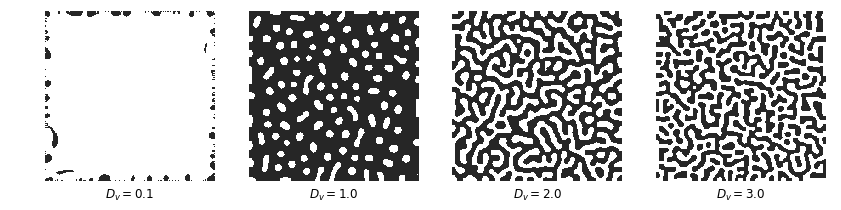
\includegraphics[width=\linewidth]{diffusivity.png}
  \caption{Figure 1: Varying Diffusivity}
  \label{fig:dv}
\end{figure}

Next we tested the assertion that the width of the stripes in the Turing pattern varies with changes in the timescale $\gamma$, where a larger $\gamma$ is expected to result in thinner stripes. The simulations in Fig. 2 confirm this.

\begin{figure}[H]
  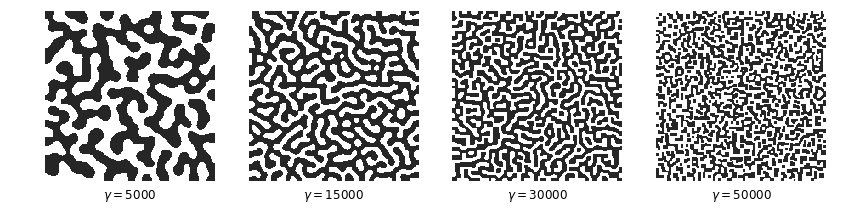
\includegraphics[width=\linewidth]{timescale.png}
  \caption{Figure 2: Varying Timescale}
  \label{fig:gamma}
\end{figure}

Most importantly, Garfinkel et al. describe a qualitative variation in the appearing patterns depending on the magnitude of the external inhibition S. Garfinkel described this in more rigorous terms in []. We were indeed able to confirm the distinct types of patterns across the parameter space. Varying the parameter $S$ from 0 to 0.5 we discovered that the system exhibited largely uniform states with holes and spots at the low and high end of the interval, respectively. In the range between we observed the appearance of a negative pattern that inverted around the value $S=0.125$ to display a positive labyrnth pattern, transitioning through a region (~[0.3,0.4]) displaying fragmented stripes into spots.

\begin{figure}
  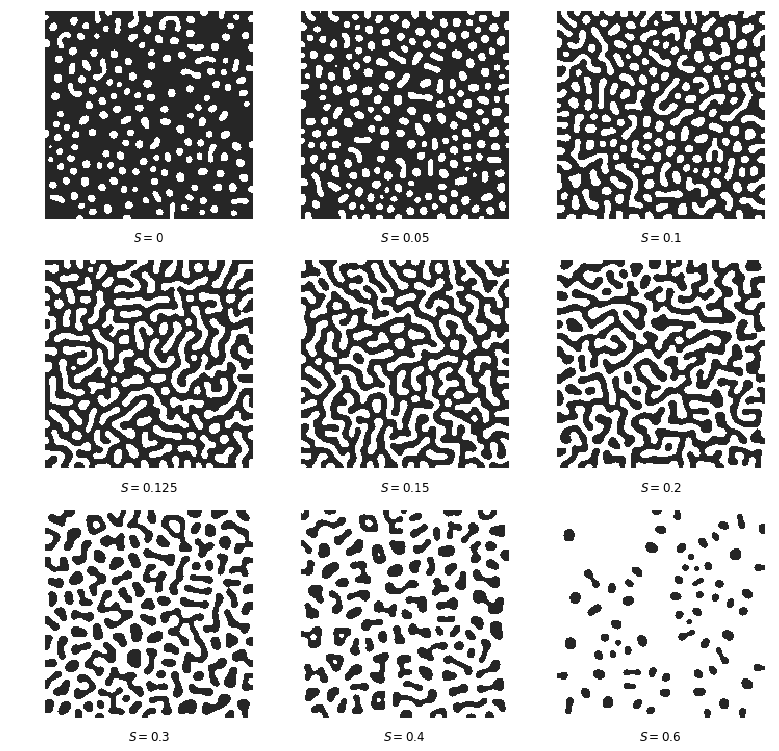
\includegraphics[width=\linewidth]{inhibition.png}
  \caption{Figure 1: Varying external inhibition}
  \label{fig:s}
\end{figure}

\end{document}
